\documentclass[../../document.tex]{subfiles}

\begin{document}
    \section{Linear Context-Free Rewriting Systems}
    In linear context-free rewriting systems (\abrv{lcfrs}), each rule composes a tuple of strings from arguments that are string tuples as well.
    The first definition formalizes the notation for such functions using binary variables that determine an argument (subscript) and one of its components (superscript).
    The sets of compositions are restricted such that the variables occur ordered according to their sub- and superscripts, and no variables for consecutive components of the same argument occur next to each other.
    These restrictions enforce a normal form for \abrv{lcfrs} that matches the properties of grammars extracted from treebanks.
    The normal form itself, however, is not restrictive: For every \abrv{lcfrs}, there is an equivalent \abrv{lcfrs} in normal form. [\citealp[Lem.~2.2]{SekMatFujKas91}; \citealp[Def.~7.2]{Kal10}]

    \begin{definition}[Compositions]\label{def:lcfrs:comp}
        We fix a set of variables \(\X = \big\{ \x_i^j \mid i, j \in \DN_+ \big\}\) and the \(\DN_+^*\)-indexed family of finite subsets \(\X_{s_1\cdots s_k} = \big\{ \x_i^j \mid i \in [k], j \in [s_i] \big\}\) for each \(k \in \DN\), and \(s_1, \ldots, s_k \in \DN_+\).
        Let \(\varSigma\) be a finite set disjoint from \(\X\).
        The family of \abrv{lcfrs} \deflab<\lcfrs>[lcfrs:comp]{composition}[compositions]\todo{define one composition and then the sets of compositions} over \(\varSigma\), denoted by \(\C^\varSigma\), is the \(\DN_+^+\)-indexed family over sets of non-empty sequences over strings in \((\varSigma \cup \X)^+\) such that for each \(k \in \DN\) and \(s_1, \ldots, s_k, s \in \DN_+\), the set \(\C^\varSigma_{s_1 \cdots s_k s}\) contains each sequence \(u_1, \ldots, u_s \in (\varSigma \cup \X_{s_1 \cdots s_k})^+\) of length \(s\) such that
        \begin{compactenum}
            \item each variable in \(\X_{s_1 \cdots s_k}\) occurs exactly once in the string \(u_1 \cdots u_s\),
            \item for each \(i \in [k-1]\), the variable \(\x_i^1\) occurs to the left of \(\x_{i+1}^1\) in the string \(u_1 \cdots u_s\),
            \item for each \(i \in [k]\) and \(j \in [s_i-1]\), the variable \(\x_i^j\) occurs to the left of \(\x_i^{j+1}\) in the string \(u_1 \cdots u_s\),
            \item there are no \(i \in [k]\) and \(j \in [s_i-1]\) such that \(\x^j_i\x^{j+1}_i\) is a subsequence in any of \(u_1, \ldots, u_s\).
        \end{compactenum}
        We associate the identifier \(\C^\varSigma\) with the set of all \abrv{lcfrs} compositions \[
        \bigcup_{k \in \DN, s_1, \ldots, s_k, s \in \DN_+} \C^{\varSigma}_{s_1 \cdots s_k s} \text{.}
        \]

        We associate a function, denoted by \(\sem{(u_1, \ldots, u_s)}\), from \(k\) string tuples, where the \(i\)-th tuple is of length \(s_i\), to a string tuple of length \(s\) with each composition in \((u_1, \ldots, u_s) \in \C^\varSigma_{(s_1\cdots s_k s)}\).
        Given the arguments \(\big(v_i = (v_i^j \mid j \in [s_i]) \mid i \in [k]\big)\), the result is the string tuple \(
        \sem{(u_1, \ldots, u_s)}(v_1, \ldots, v_k) = (u_1[\phi], \ldots, u_s[\phi])
        \) where \(\phi\) is the \(\X_{s_1 \cdots s_k}\)-indexed family with \(\phi_{x_i^j} = v_i^j\).
        Intuitively, this function replaces each occurring variable of the form \(\x_i^j\) in \(u_1, \ldots, u_s\) with the \(j\)-th component of the \(i\)-th argument.
    \end{definition}

    \begin{example}\label{ex:lcfrs:comp}
        Consider an alphabet \(\Sigma=\{\tn{A}, \tn{hearing}, \tn{is}, \tn{scheduled}, \tn{on}, \tn{the}, \tn{issue}, \tn{today}\}\) and the following compositions:
        \begin{align*}
            c_1 &= (\tn{A}), & c_2 &= (\tn{today}), & c_3 &= (\tn{issue}) && \in \C^\Sigma_{(1)} \\
            c_4 &= (\tn{the} \, \x_1^1), & c_5 &= (\x_1^1 \, \tn{hearing}) & & && \in \C^\Sigma_{(1\,1)} \\
            c_6 &= (\x_1^1 \, \tn{is} \, \x_1^2) && && && \in \C^\Sigma_{(2\,1)} \\
            c_7 &= (\x_1^1, \tn{on} \, \x_2^1) && && && \in \C^\Sigma_{(1\,1\,2)}   \\
            c_8 &= (\x_1^1, \tn{scheduled} \, \x_1^2 \, \x_2^1) && && && \in \C^\Sigma_{(2\,1\,2)}
        \end{align*}

        The subscript indexing the family of compositions \(\C^\Sigma\) determines the arity of the associated functions.
        E.g.\@ \(\sem{c_1} \in \C^\Sigma_{(1)}\) takes no arguments (it is constant) and yields a single string,
        \(\sem{c_8} \in \C^\Sigma_{(2\,1\,2)}\) takes two arguments, a sequence over strings of length 2 and 1, and gives a sequence of length 2 as a result.
        For example:
        \begin{multline*}
            \sem{c_8}\Big( \; \big( \tn{A hearing}, \: \tn{on the issue} \big), \, \big( \tn{today} \big) \; \Big)
            \\= \big( \tn{A hearing}, \: \tn{scheduled on the issue today} \big)
        \end{multline*}

        The functions may form terms, e.g.
        \begin{align*}
            \sem{c_7}\Big( \; \sem{c_5}\big(\,\sem{c_1}()\,\big), \: \sem{c_4}\big(\,\sem{c_3}()\,\big) \; \Big)
            =& \sem{c_7}\Big( \; \sem{c_5}\big(\tn{A}\big), \: \sem{c_4}\big(\tn{issue}\big) \; \Big) \\
            =& \sem{c_7}\Big( \; (\tn{A hearing}), \: (\tn{the issue}) \; \Big) \\
            =& (\tn{A hearing}, \: \tn{on the issue})
        \end{align*}
    \end{example}

    \begin{definition}[\abrv{Lcfrs} Grammar]
        A \deflab[lcfrs]{\lcfrs} (\abrv{lcfrs})%
        \defabrv{\lcfrs}{\abrv{lcfrs}}
        is a tuple \(G=(N, \varSigma, S, R)\) where
        \begin{compactenum}
            \item \(N\) is a finite set (\emph{nonterminals}),
            \item \(\varSigma\) is an alphabet (\emph{terminals}),
            \item \(S \in N\) (initial non-terminal),
            \item \(R\) is a finite subset of \(N \times \C^\varSigma \times N^*\) (\deflab<\lcfrs>{rule}[rules]),\todo{define set of rules over \(N, \varSigma\) and families} and
            \item there is an implicit positive integer \(\fanout(A) \in \DN_+\), called the \deflab<\lcfrs>[lcfrs:fo]{fanout} for each nonterminal \(A \in N\), such that
            for each \((A, c, B_1\cdots B_k) \in R\), the \abrv{lcfrs} composition \(c\) is an element of \(\C^\varSigma_{\fanout(B_1) \cdots \fanout(B_k) \fanout(A)}\).
        \end{compactenum}

        Rules are denoted in the form \(A \to c\,(B_1, \ldots, B_k)\) instead of \((A, c, B_1 \cdots B_k)\); \(A\) is called the left-hand side (\abrv{lhs}) nonterminal and \(B_1, \ldots B_k\) are the right-hand side (\abrv{rhs}) nonterminals, \(c\) is the composition of the rule.
        The natural \(k\) is the \deflab<\lcfrs!rule>[lcfrs:rk]{rank} of the rule; the \emph{rank} of the grammar \(G\) is the maximum rank occurring in the rules of \(G\).
    \end{definition}

    \begin{definition}[\abrv{Lcfrs} Grammar Forms]
        We distinguish rules and grammars of the following form:
        \begin{compactitem}
            \item Rules of rank zero, one and two are called \deflab<\lcfrs!rule>{nullary}, \deflab<\lcfrs!rule>{unary} and \deflab<\lcfrs!rule>{binary}, respectively.
            \item Lcfrs containing only nullary, unary and binary rules are called \deflab<\lcfrs>[lcfrs:bin]{binary}.
            \item Rules whose composition contains exactly one terminal in \(\varSigma\) are called \deflab<\lcfrs!rule>[lcfrs:lex]{lexical}.
            \item Lcfrs containing only lexical rules are called \deflab<\lcfrs>{lexical}.
            \item Rules whose composition contain no terminal at all are called \deflab<\lcfrs!rule>{non-lexical}.
            \item Lcfrs that contain only lexical nullary rules and non-lexical rules of rank \(\ge 1\) are called \deflab<\lcfrs>[lcfrs:simple]{simple}.
        \end{compactitem}
    \end{definition}

    \begin{example}[Continues \cref{ex:lcfrs:comp}]\label{ex:lcfrs:rules}
        Consider the alphabet \(\mathrm{N} = \{\nt{vp}, \nt{vp}_2, \nt{np}, \nt{np}_2, \nt{pp}, \nt{np}^\nt{L}\}\) of nonterminal symbols and the \abrv{lcfrs} \(\mathrm{G} = (\mathrm{N}, \Sigma, \nt{vp}, \mathrm{R})\) with
        \begin{align*}
            \mathrm{R} = \big\{\;
            \nt{n}^\nt{l} &\to (\tn{A})\:(), &\nt{n} &\to (\tn{issue})\:(), &\nt{n} &\to (\tn{today})\:(), &\\
            \nt{n} &\to (\x_1^1 \, \tn{hearing})\:(\nt{n}^\nt{l}), &\nt{p} &\to (\tn{the}\,\x_1^1)\:(\nt{n}), \\
            \nt{n}_2 &\to (\x_1^1, \tn{on} \, \x_2^1)\:(\nt{n}, \nt{p}), \\
            \nt{v}_2 &\to (\x_1^1, \tn{scheduled} \, \x_1^2 \, \x_2^1)\:(\nt{n}_2, \nt{n}), \\
            \nt{v} &\to (\x_1^1 \, \tn{is} \, \x_1^2)\:(\nt{v}_2)
            &&&&&\;\big\}
        \end{align*}
        The fanout for each nonterminal \(A\) determines the length of the composition with \abrv{lhs} \(A\) and the number of variables if \(A\) occurs in the \abrv{rhs} nonterminals of a rule.
        In the above example, the nonterminal symbols with subscript \(_2\), i.e.\@ \(\nt{n}_2\) and \(\nt{v}_2\), are of fanout 2, and all others of fanout 1.
        The composition of the rule \(\nt{v}_2 \to (\x_1^1, \tn{scheduled} \, \x_1^2 \, \x_2^1)\:(\nt{n}_2, \nt{n})\) is of length \(\fanout(\nt{v}_2) = 2\) and there are \(\fanout(\nt{n}_2) = 2\) variables for the first \abrv{rhs} nonterminal and \(\fanout(\nt{n}) = 1\) for the second.
        \todo{G is lexical, example for simple lcfrs?}
    \end{example}

    \begin{definition}[Derivation]
        Let us consider an lcfrs \(G = (N, \varSigma, S, R)\).
        An \abrv{lcfrs} \deflab<\lcfrs>[lcfrs:deriv]{derivation} is a tree over rules in \(\T_R\) that suffices the following conditions:
        \begin{compactitem}
            \item Each leaf is equipped with a nullary rule as symbol.
            \item Each inner node is a rule with the same amount of \abrv{rhs} nonterminals as children in the tree such that the \(i\)-th \abrv{rhs} nonterminal is the \(i\)th child's \abrv{lhs} nonterminal.
        \end{compactitem}
        The set of all \abrv{lcfrs} derivations is denoted by \(\derivs^R\).
        We identify this set with the \(N\)-indexed partition of \(\derivs^R\) that assigns each nonterminal \(A\) to the derivations whose root is equipped with \abrv{lhs} \(A\).
    \end{definition}

    \begin{definition}[Yield and Parse]
        Consider a derivation \(d\) in \(\derivs^R_A\) of the form \(d = r\,(d_1, \ldots, d_k)\) where the root \(r\) is of the form \(A \to c\,(B_1, \ldots, B_k)\).
        The \deflab<\lcfrs!derivation>[lcfrs:yd]{yield} of \(d\) is defined recursively: \(\yield(d) = \sem{c}(\yield(d_1), \ldots, \yield(d_k))\).
        For the definition of the parse of \(d\), let us consider the sequences of terminal symbols \(w_1, \ldots, w_{k+1} \in \varSigma^*\) such that,
        \begin{compactitem}
            \item \(w_1\) is the sequence of terminal symbols occurring before the variable \(\x_1^1\) in \(c\),
            \item for each \(i \in \{2, \ldots, k\}\), \(w_i\) is the sequence of terminal symbols occurring between the variables \(\x_{i-1}^1\) and \(\x_i^1\) in \(c\), and
            \item \(w_{k+1}\) is the sequence of terminal symbols occurring after the variable \(\x_k^1\) in \(c\).
        \end{compactitem}
        Then the \deflab<\lcfrs!derivation>[lcfrs:parse]{parse} of \(d\) is the tree \[
        \parse(d) = A(w_1, \parse(d_1), w_2, \parse(d_2), \ldots, w_k, \parse(d_k), w_{k+1}) \text{.}
        \]
    \end{definition}

    \begin{example}[Continues \cref{ex:lcfrs:comp,ex:lcfrs:rules}]\label{ex:lcfrs:deriv}
        Let's consider the two trees illustrated below, the left one \(d\) is a tree over rules in the \abrv{lcfrs} \(\mathrm{G} = (N, \Sigma, \nt{v}, R)\), the right one is an element in \(\T_N(\Sigma)\).
        Its root has the \abrv{lhs} \(\nt{n}_2\), the tree is an element of \(\derivs^R_{\nt{n}_2}\).
        The yield of \(d\) is term over compositions computed in \cref{ex:lcfrs:comp}: \(\yield(d) = (\tn{A hearing}, \: \tn{on the issue})\).
        The parse of \(d\) is illustrated to the right of \(d\).

        \null\hfill
        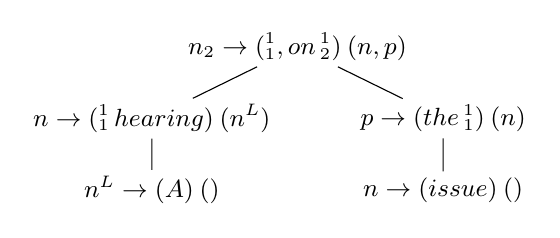
\begin{tikzpicture}[level distance=6ex, font=\small, sibling distance=3.7cm, inner sep=2pt]
            \node {\(\nt{n}_2 \to (\x_1^1, \tn{on} \, \x_2^1)\:(\nt{n}, \nt{p})\)}
            child {node {\(\nt{n} \to (\x_1^1 \, \tn{hearing})\:(\nt{n}^\nt{L})\)}
                child {node {\(\nt{n}^\nt{L} \to (\tn{A})\:()\)}}}
            child {node {\(\nt{p} \to (\tn{the}\,\x_1^1)\:(\nt{n})\)}
                child {node {\(\nt{n} \to (\tn{issue})\:()\)}}};
        \end{tikzpicture}
        \hfill
        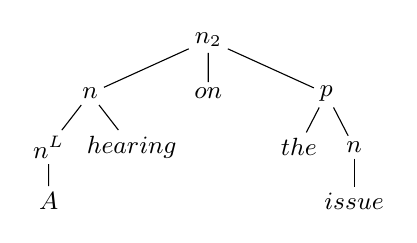
\begin{tikzpicture}[level distance=4.5ex, font=\small, inner sep=2pt]
            \node {\(\nt{n}_2\)}
            child {node {\(\nt{n}\)}
                [sibling distance=3em]
                child {node {\(\nt{n}^\nt{L}\)}
                    child { node {\(\tn{A}\)}}}
                child {node {\(\tn{hearing}\)}}}
            child {node {\(\tn{on}\)}}
            child {node {\(\nt{p}\)}
                [sibling distance=2em]
                child {node {\(\tn{the}\)}}
                child {node {\(\nt{n}\)}
                    child { node {\(\tn{issue}\)}}}};
        \end{tikzpicture}
        \hfill\null
    \end{example}
\end{document}